\chapter{Creating an \rtd\ project}
\label{cha:creating-rtdruid-project}

Following the standard Eclipse convention, the creation of a new \rtd\
project starts from the wizard for project creation, accessible in
several ways, such as, for example, by pressing the ``File'' button in
the menubar and then the ``New'' and the ``Project'' buttons in
sequence (see Figure \ref{fig:rtdruid-project-new}).

\begin{figure}
  \begin{center}
    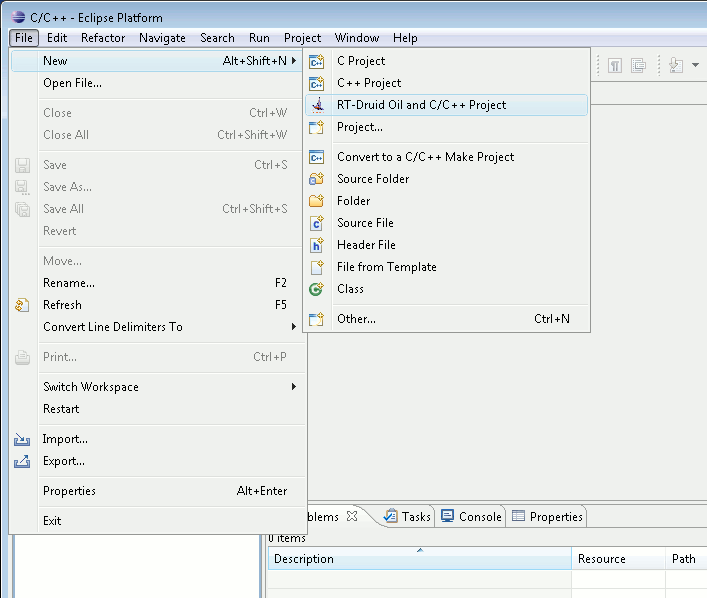
\includegraphics[width=8cm, bb=0 0 707 598]{images/project_new.png}
  \end{center}
  \caption{Activating the ``New Project'' Wizard.}
  \label{fig:rtdruid-project-new}
\end{figure}

After that, the wizard asks for a project template (see Figure
\ref{fig:rtdruid-project-template}), which is a pre-built application
that you can use, and after that for the project name and optionally
for the name of the home folder for the project. The use of spacing
characters in the project name is {\bf strongly discouraged} and
strictly forbidden for the names of all files inside the project
folder, since they would create problems with the
\file{make} and \file{gcc} tools when compiling a project, since (\file{make}
and \file{gcc} treat spaces as separators inside lists of file names
(see Figure \ref{fig:rtdruid-project-name}).

\begin{figure}
  \begin{center}
    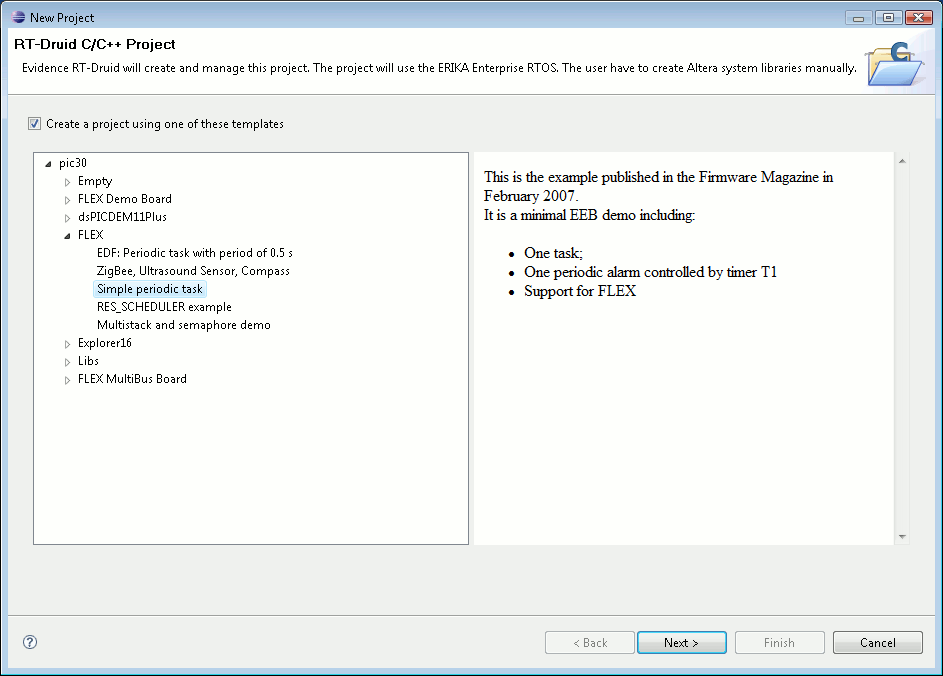
\includegraphics[width=8cm, bb=0 0 943 676]{images/project_template.png}
  \end{center}
  \caption{Choosing a template application for your new \rtd\ Project.}
  \label{fig:rtdruid-project-template}
\end{figure}

\begin{figure}
  \begin{center}
    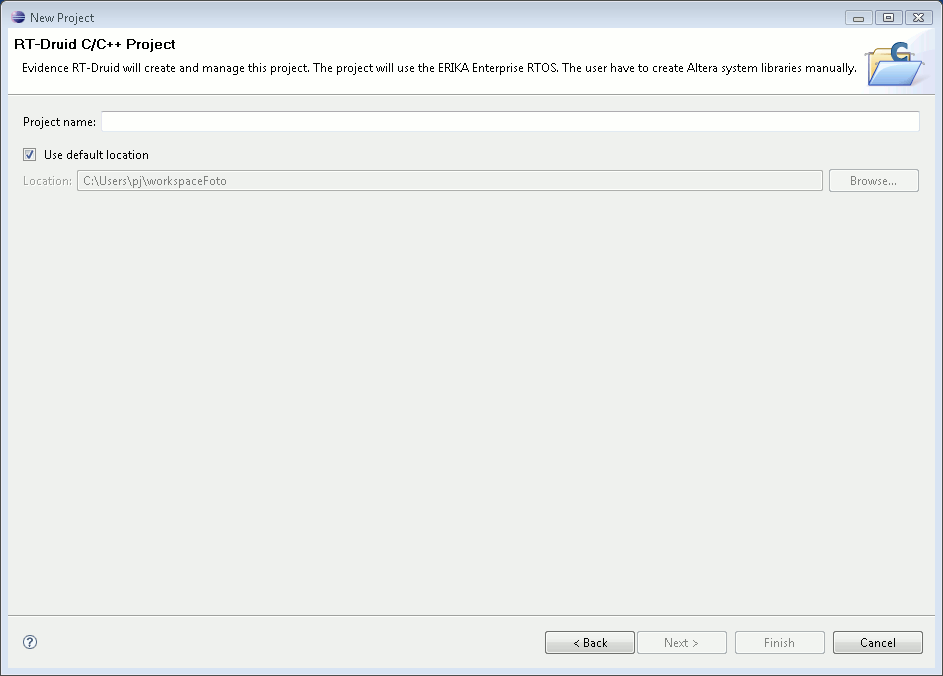
\includegraphics[width=8cm, bb=0 0 943 676]{images/project_name.png}
  \end{center}
  \caption{Choosing a  meaningful name for your new \rtd\ Project.}
  \label{fig:rtdruid-project-name}
\end{figure}

Once these steps are completed, the project is created and a OIL
configuration file template is automatically generated and inserted
into the project.

To edit the OIL File, just double click on it in the Navigation
sidebar, and a dedicated OIL Editor will appear.






